\section{Prepara Tú Documento Antes de Estilizarlo} \label{sec:prep_docum}

Antes de empezar a dar formato a su trabajo, primero escriba y guarde el contenido como un archivo de texto independiente. Antes de formatear, complete toda la edición de contenido y organización. En las secciones \ref{subsec:abrev_acron}--\ref{subsec:error_comun} que encontrará más información sobre corrección, ortografía y gramática. \par

Mantenga los archivos de texto y gráficos separados hasta que el texto haya sido formateado y estilizado. No numere los encabezados de los textos, ya lo hará {\LaTeX}.

\subsection{Abreviaciones y Acrónimos} \label{subsec:abrev_acron}

Defina las abreviaturas y siglas la primera vez que sean usadas en el texto, incluso después de haberlas definido en el resumen. Abreviaturas como IEEE, SI, MKS, CGS, ac, dc, y rms no es necesario definirlas. No utilice abreviaturas en el título o los encabezamientos a menos que sean inevitables.


\subsection{Unidades} \label{subsec:unid}

\begin{itemize}
    \item Utilice el SI (MKS) o el CGS como unidades primarias. (Unidases SI son recomiendadas). Pueden utilizarse unidades inglesas secundarias (entre paréntesis). Una excepción sería el uso de unidades inglesas como identificadores en el comercio, como ``3,5 pulgadas''.
    \item Evite combinar unidades SI y CGS, como corriente en amperios y campo magnético en oersteds. Esto confusión porque las ecuaciones no se equilibran dimensiones. Si debe utilizar unidades mixtas, indique claramente las unidades de cada cantidad que utilices en una ecuación
    \item No mezcles grafías completas y abreviaturas de unidades: ``$Wb/{m}^2$'' o ``webers por metro cuadrado'', no ``$webers/{m}^2$''. Deletrea las unidades cuando aparezcan en el texto: ``. . . unos cuantos henrios'', no ``. . . unas cuantas H''.
    \item Utilice un cero antes de los decimales: ``0,25'', no ``,25''. Utilice ``$cm^3$'', no ``cc'').
\end{itemize}

\subsection{Ecuaciones} \label{subsec:ecuac}

Numera las ecuaciones consecutivamente. Para que tus ecuaciones sean más compactas, puedes utilizar el solidus ( / ), la función exp o los exponentes adecuados. Ponga en cursiva los símbolos romanos para cantidades y variables, pero no los símbolos griegos. Utilice un guión largo en lugar de un guión para el signo menos. Puntúe las ecuaciones con comas o puntos cuando formen parte de una frase, como en:
\begin{equation}
    \label{eq:gamma}
    a+b=\gamma
\end{equation}

Asegúrate de que los símbolos de tu ecuación han sido definidos antes o inmediatamente después de la ecuación. Utiliza ``\eqref{eq:gamma}'', no ``Ec. \eqref{eq:gamma}'' ni ``ecuación \eqref{eq:gamma}'', excepto al principio de una frase: ``La ecuación \eqref{eq:gamma} es...''.


\subsection{Consejos Epecificos para {\LaTeX}} \label{subsec:cons_latex}

Utilice referencias cruzadas "suaves" (por ejemplo, \verb|\eqref{Eq})| en lugar de referencias "duras" (por ejemplo, \verb|(1)|). Así podrá combinar secciones, añadir ecuaciones o cambiar el orden de las figuras o citas sin tener que revisar el archivo línea por línea. \par

Por favor, no utilices el entorno de ecuación \verb|{eqnarray}|. Utilice \verb|{align}| o \verb|{IEEEeqnarray}| en su lugar. El entorno \verb|{eqnarray}| deja espacios antiestéticos alrededor de los símbolos de relación. \par

Tenga en cuenta que el entorno \verb|{subequations}| en {\LaTeX} incrementará el contador principal de ecuaciones incluso cuando no se muestren números de ecuaciones. Si olvida esto, puede escribir un artículo en el que los números de ecuación salten de (17) a (20), haciendo que los editores se pregunten si ha descubierto un nuevo método de conteo. \par

{\BibTeX} no funciona por arte de magia. No obtiene los datos bibliográficos de la nada, sino de archivos .bib. Si utiliza {\BibTeX} para elaborar una bibliografía, deberá enviar los ficheros .bib. \par

{\LaTeX} no puede leer su mente. Si asigna la misma etiqueta a una subsubsección y a una tabla, puede encontrar que la Tabla \ref{tab:estil_tab} ha sido referenciada como Tabla IV-B3. \par

El comando \verb|\label| antes del comando que actualiza el contador que se supone que debe utilizar, la etiqueta tomará el último contador al que se hace referencia cruzada. En particular, un comando \verb|\label| no debe ir antes de la leyenda de una figura o una tabla. \par

No utilice \verb|\nonumber| dentro del entorno \verb|{array}|. No detendrá los números de ecuación dentro de \verb|{array}| (no habrá ninguno de todos modos) y podría detener un número de ecuación deseado en la ecuación circundante.

\subsection{Algunos Errores Comunes} \label{subsec:error_comun}

\begin{itemize}
    \item La palabra ``datos'' es plural, no singular.
    \item El subíndice para la permeabilidad del vacío $\mu_{0}$, y otras constantes científicas comunes, es cero con subíndice y no una letra ``o'' minúscula.
    \item En inglés americano, las comas, los puntos y coma, los puntos, los signos de interrogación y exclamación se sitúan dentro de las comillas sólo cuando se cita un pensamiento o nombre completo, como un título o una cita completa. Cuando se utilizan comillas, en lugar de negrita o cursiva, para resaltar una palabra o frase, la puntuación debe aparecer fuera de las comillas. Una frase o afirmación entre paréntesis al final de una oración se puntúa fuera del paréntesis de cierre (así). (Una frase parentética se puntúa dentro del paréntesis).
    \item Un gráfico dentro de otro gráfico es un ``inserto'', no una ``inserción''. La palabra alternativamente es preferible a la palabra ``alternativamente'' (a menos que realmente quieras decir algo que alterna).
    \item No utilice la palabra ``esencialmente'' para referirse a ``aproximadamente'' o ``efectivamente''.
    \item En el título de su artículo, si las palabras ``que utiliza'' pueden sustituir con precisión a la palabra ``utilizando'', escriba la ``u'' en mayúsculas; si no, siga utilizando minúsculas.
    \item Ten en cuenta los distintos significados de los homófonos ``afectar'' y ``efecto'', ``complemento'' y ``cumplido'', ``discreto'' y ``discreto'', ``principal'' y ``principio''.
    \item No confunda ``implicar'' e ``inferir''.
    \item El prefijo ``non'' no es una palabra a la que modifica, normalmente sin guión.
    \item No hay punto después del ``et'' en la abreviatura latina ``et al.''.
    \item La abreviatura ``i.e.'' significa ``es decir'', y la abreviatura ``e.g.'' significa ``por ejemplo''.
\end{itemize}
Un excelente manual de estilo para escritores científicos es \cite{young1989}.

\subsection{Autores y Afiliaciones} \label{subsec:autor_afilia}

\textbf{El archivo de clase está diseñado para seis autores, aunque no limitado a ellos.} Se requiere un mínimo de un autor para todos los artículos de conferencias. Los nombres de los autores deben enumerarse empezando de izquierda a derecha y bajando a la línea siguiente. Esta es la secuencia de autores que se utilizará en futuras citas y por los servicios de indexación. Los nombres no deben aparecer en columnas ni agrupados por afiliación. Las afiliaciones deben ser lo más sucintas posible (por ejemplo, no distinga entre departamentos de la misma organización).

\subsection{Identificar Títulos} \label{subsec:ident_titul}

Los títulos o encabezamientos son elementos organizativos que guían al lector a través del documento. Existen dos tipos: los encabezamientos de componente y los encabezamientos de texto. \par

Los encabezamientos de los componentes identifican los distintos elementos de su documento y no están subordinados tópicamente entre sí. Por ejemplo, los agradecimientos y las referencias, para los que el estilo correcto es el "Título 5". Utilice "Pie de figura" para los pies de figura y "Cabecera de tabla" para el título de la tabla. Los encabezamientos seguidos, como "Resumen", requerirán que aplique un estilo (en este caso, cursiva) además del estilo proporcionado por el menú desplegable para diferenciar el encabezamiento del texto. \par

Los encabezamientos de texto organizan los temas sobre una base jerárquica y relacional. Por ejemplo, el título del artículo es el encabezamiento principal porque todo el material posterior se relaciona con este tema y lo desarrolla. Si hay dos o más subtemas, se utilizará el siguiente nivel (números romanos en mayúscula) y, a la inversa, si no hay al menos dos subtemas, no se introducirá ningún subtítulo.

\subsection{Figuras y Tablas} \label{subsec:fig_tab}

\subsubsection{Posición de Figuras y Tablas} \label{subsubsec:posic_fig_tab}

Coloque las figuras y tablas en la parte superior e inferior de las columnas. Evite colocarlas en medio de las columnas. Las figuras y tablas grandes pueden abarcar ambas columnas. Las leyendas de las figuras deben ir debajo de las figuras; las cabezas de las tablas deben aparecer encima de las tablas. Inserte las figuras y tablas después de citarlas en el texto. Utilice la abreviatura ``Fig. \ref{fig:ejm_fig}'', incluso al principio de una frase.

\begin{table}[!htb]
    \caption{Estilos de Tabla}
    \label{tab:estil_tab}
    \Centering
    \begin{tabular}{%
    |>{\Centering\arraybackslash}p{3em}
    |>{\Centering\arraybackslash}p{10em}
    |>{\Centering\arraybackslash}p{4em}
    |>{\Centering\arraybackslash}p{4em}|
}

    \hline
    \multirow{2}{*}{\textbf{\makecell[tc]{Table \\ Head}}} & \multicolumn{3}{c|}{\textbf{Table Column Head}} \\
    \cline{2-4}
    
    & \textbf{Table column subhead} & \textbf{Subhead} & \textbf{Subhead} \\
    \hline

    copy & More table copy$^{\mathrm{a}}$ & & \\
    \hline

    \multicolumn{4}{l}{$^{\mathrm{a}}$Sample of a Table footnote.}

\end{tabular}
\end{table}

\begin{figure}[!htb]
    \Centering
    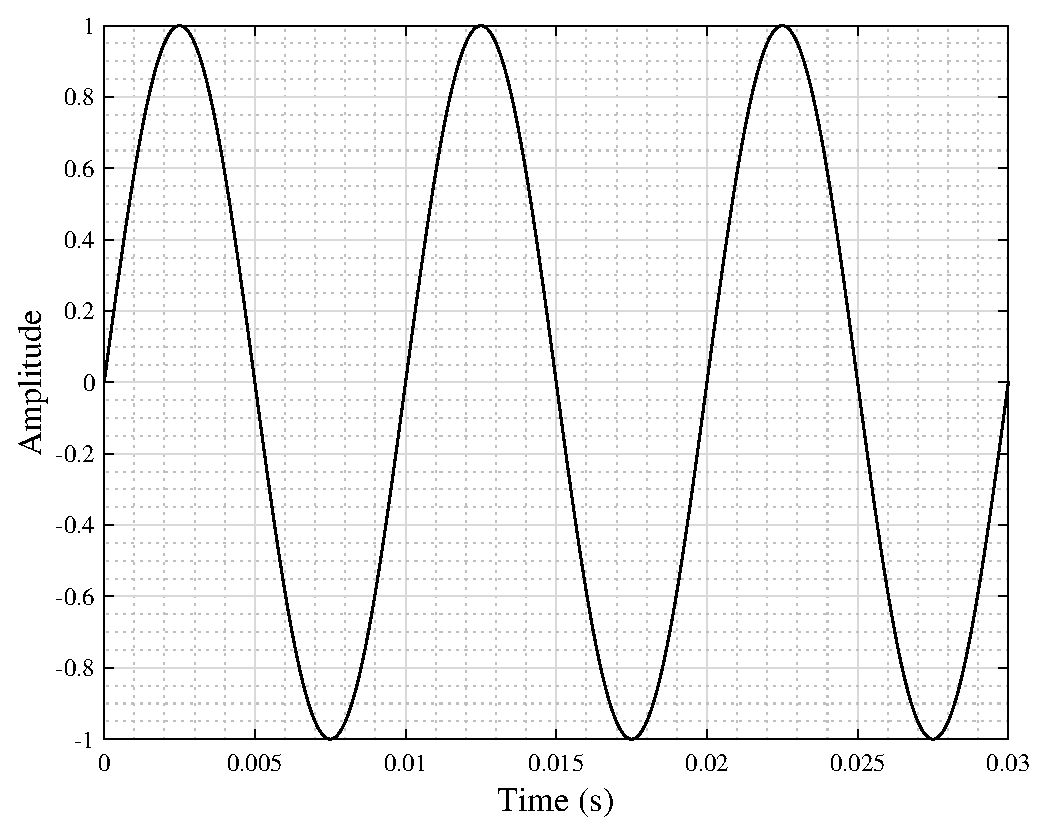
\includegraphics[width=0.9\columnwidth]{Figuras/senoide.eps}
    \caption{Ejemplo de pie de figura}
    \label{fig:ejm_fig}
\end{figure}

Etiquetas de las figuras: Utilice Times New Roman de 8 puntos para las etiquetas de las figuras. Utilice palabras en lugar de símbolos o abreviaturas para no confundir al lector. Por ejemplo, escriba la cantidad ``Magnetización'' o ``Magnetización, M'', no sólo ``M''. Si incluye unidades en la etiqueta, preséntelas entre paréntesis. No etiquete los ejes sólo con unidades. En el ejemplo, escriba ``Magnetización ($A/m$)'' o ``Magnetización A[m(1)]'', no sólo ``$A/m$''. No etiquetes los ejes con una relación de cantidades y unidades. Por ejemplo, escriba ``Temperatura (K)'', no ``Temperatura/K''.

\subsection{Códigos} \label{sec:cod_algor}

La gráfica senoidal representada en la figura \ref{fig:ejm_fig} se generó con el algoritmo que se muestra en el código \ref{lst:ejm1}. El argumento de entrada \verblst{matlabstyle}{'Senoide'} especifica el nombre del archivo y el argumento \verblst{matlabstyle}{'eps'} exporta la imagen como archivo vectorial ``.eps'' nivel 3 a blanco y negro.

\lstinputlisting[%
    style = matlabstyle,
    caption = Ejemplo de pie de código.,
    label = lst:ejm1,
    belowskip = 0pt,
]{Codigos/senoide.m}